\documentclass{article}
\usepackage{ctex}
\title{编译原理 作业4}
\author{} 
\date{}
\usepackage[a4paper,left=10mm,right=10mm,top=15mm,bottom=15mm]{geometry} 
\usepackage{graphicx} 
\usepackage{makecell}
\usepackage[linguistics]{forest}

\begin{document}
\section*{5.1}
\noindent 
根据题目中所给的文法$G_1$,有如下推导$E\Rightarrow E+T\Rightarrow E+T*F$.\\
因此$E+T*F$是$G_1$的句型.\\
这一句型有短语: $E+T*F, T*F$,直接短语: $T*F$,句柄: $T*F$.\\
\section*{5.2}
\noindent 
\textbf{(1)}最左推导:\\
$S\Rightarrow(T)\Rightarrow(T, S)\Rightarrow(S, S)\Rightarrow(a, S)\Rightarrow(a,(T))
\Rightarrow (a, (T, S))\Rightarrow (a, (S, S))\Rightarrow (a,(a,S))\Rightarrow (a,(a,a))$\\
$S\Rightarrow (T,S)\Rightarrow ((T), S)\Rightarrow((T,S), S) \Rightarrow ((T,S,S), S)
\Rightarrow((S,S,S), S) \Rightarrow (((T), S, S), S)\Rightarrow (((T, S), S, S), S)
\Rightarrow(((S, S)S, S), S) \Rightarrow(((a, S), S, S), S) \Rightarrow(((a, a), S, S), S) 
\Rightarrow (((a, a), \^{}, S), S)\Rightarrow(((a, a), \^{} , (T)), S) 
\Rightarrow (((a, a), \^{}, (S)), S)\Rightarrow (((a, a), \^{}, (a)), S)
\Rightarrow (((a, a), \^{}, (a)), a)$\\
最右推导:\\
$S\Rightarrow(T)\Rightarrow(T, (T))\Rightarrow (T, (T, S))\Rightarrow (T, (T, a))
\Rightarrow (T, (S, a))\Rightarrow (T, (S, a))\Rightarrow (T, (a, a))\Rightarrow (S, (a, a))\Rightarrow (a,(a,a))$\\
$S\Rightarrow (T,S)\Rightarrow (T, a)\Rightarrow (S, a)\Rightarrow ((T), a)
\Rightarrow ((T, S), a)\Rightarrow ((T, (T)), a)\Rightarrow ((T, (S)), a)
\Rightarrow ((T, (a)), a)\Rightarrow ((T,S, (a)), a)\Rightarrow((T,\^{}, (a)), a)
\Rightarrow((S,\^{}, (a)), a) \Rightarrow(((T),\^{}, (a)), a)
\Rightarrow(((T, S),\^{}, (a)), a)\Rightarrow(((T, a),\^{}, (a)), a)
\Rightarrow(((S, a),\^{}, (a)), a)\Rightarrow(((a, a), \^{}, (a)), a)$\\
\textbf{(2)}规范规约过程如下所示:\\
$(((\underline{\textbf{a}},a),\^{},(a)),a)$\\
$(((\underline{\textbf{S}},a),\^{},(a)),a)$\\
$(((T,\underline{\textbf{a}}),\^{},(a)),a)$\\
$(((\underline{\textbf{T, S}}),\^{},(a)),a)$\\
$(((\underline{\textbf{T}}),\^{},(a)),a)$\\
$((\underline{\textbf{S}},\^{},(a)),a)$\\
$((T,\^{},(a)),a)$\\
$((\underline{\textbf{T, S}},(a)),a)$\\
$((T,(\underline{\textbf{a}})),a)$\\
$((T,(\underline{\textbf{S}})),a)$\\
$((T,(\underline{\textbf{T}})),a)$\\
$((\underline{\textbf{T, S}}),a)$\\
$((\underline{\textbf{T}}),a)$\\
$(\underline{\textbf{S}},a)$\\
$(\underline{\textbf{T, S}})$\\
$(\underline{\textbf{T}})$\\
$S$\\
移进-规约过程如下所示:
\begin{tabbing}
    \hspace{1.5cm} \= \hspace{3cm} \= \hspace{5cm} \= \hspace{1.5cm} \= \kill
    \textbf{步骤}\>\textbf{符号栈}\>\textbf{输入串}\>\textbf{动作}\\
    0\> \#  \> $(((a,a),\^{},(a)),a)\#$ \>  \\
    
    1\> \#( \> $((a,a),\^{},(a)),a)\#$ \> 移进 \\
    
    2\> \#(( \> $(a,a),\^{},(a)),a)\#$ \> 移进 \\
    
    3\> \#((( \> $a,a),\^{},(a)),a)\#$ \> 移进 \\
    
    4\> \#(((a \> $,a),\^{},(a)),a)\#$ \> 移进 \\
    
    5\> \#(((S \> $,a),\^{},(a)),a)\#$ \> 规约 \\
    
    6\> \#(((T \> $,a),\^{},(a)),a)\#$ \> 规约 \\
    
    7\> \#(((T, \> $a),\^{},(a)),a)\#$ \> 移进 \\
    
    8\> \#(((T,a \> $),\^{},(a)),a)\#$ \> 移进 \\
    
    9\> \#(((T,S \> $),\^{},(a)),a)\#$ \> 规约 \\
    
    10\> \#(((T \> $),\^{},(a)),a)\#$ \> 规约 \\
    
    11\> \#((T) \> $,\^{},(a)),a)\#$ \> 移进 \\
    
    12\> \#((S \> $,\^{},(a)),a)\#$ \> 规约 \\
    
    13\> \#((T \> $,\^{},(a)),a)\#$ \> 规约 \\
    
    14\> \#((T, \> $\^{},(a)),a)\#$ \> 移进 \\
    
    15\> \#((T,\^{} \> $,(a)),a)\#$ \> 移进 \\
    
    16\> \#((T,S \> $,(a)),a)\#$ \> 规约 \\
    
    17\> \#((T \> $,(a)),a)\#$ \> 规约 \\
    
    18\> \#((T, \> $(a)),a)\#$ \> 移进 \\
    
    19\> \#((T,( \> $a)),a)\#$ \> 移进 \\
    
    20\> \#((T,(a \> $)),a)\#$ \> 移进 \\
    
    21\> \#((T,(S \> $)),a)\#$ \> 规约 \\
    
    22\> \#((T,(T \> $)),a)\#$ \> 规约 \\
    
    23\> \#((T,(T) \> $),a)\#$ \> 移进 \\
    
    24\> \#((T,S \> $),a)\#$ \> 规约 \\
    
    25\> \#((T \> $),a)\#$ \> 规约 \\
    
    26\> \#((T) \> $,a)\#$ \> 移进 \\
    
    27\> \#(S \> $,a)\#$ \> 规约 \\
    
    28\> \#(T \> $,a)\#$ \> 规约 \\
    
    29\> \#(T,  \> $a)\#$ \> 移进 \\
    
    30\> \#(T, a \> $)\#$ \> 移进 \\
    
    31\> \#(T,S \> $)\#$ \> 规约 \\
    
    32\> \#(T \> $)\#$ \> 规约 \\
    
    33\> \#(T) \> $\#$ \> 移进 \\
    
    34\> \#S \> $\#$ \> 规约 \\
\end{tabbing}
则语法树构建如下所示:
\begin{forest}
    [S[(T)[T[S[(T)[T[T[S[(T)[T[S[a]]][S[a]]]]][S[\text{\^{}}]]][S[(T)[S[a]]]]]]][S[a]]]]
\end{forest}

\section*{5.5}
\noindent 
\textbf{(1)}该文法的所有LR(0)项目如下所示,共11个:\\
$S'\rightarrow\cdot S$\\
$S'\rightarrow S\cdot$\\
$S\rightarrow \cdot AS$\\
$S\rightarrow\cdot A\cdot S$\\
$s\rightarrow AS\cdot $\\
$S\rightarrow\cdot b$\\
$S\rightarrow b\cdot$\\
$A\rightarrow\cdot SA$\\
$A\rightarrow S\cdot A$\\
$A\rightarrow SA$\\
$A\rightarrow\cdot a$\\
$A\rightarrow a\cdot $\\
\textbf{(2)}
NFA和DFA如下所示:\\
\begin{center}
    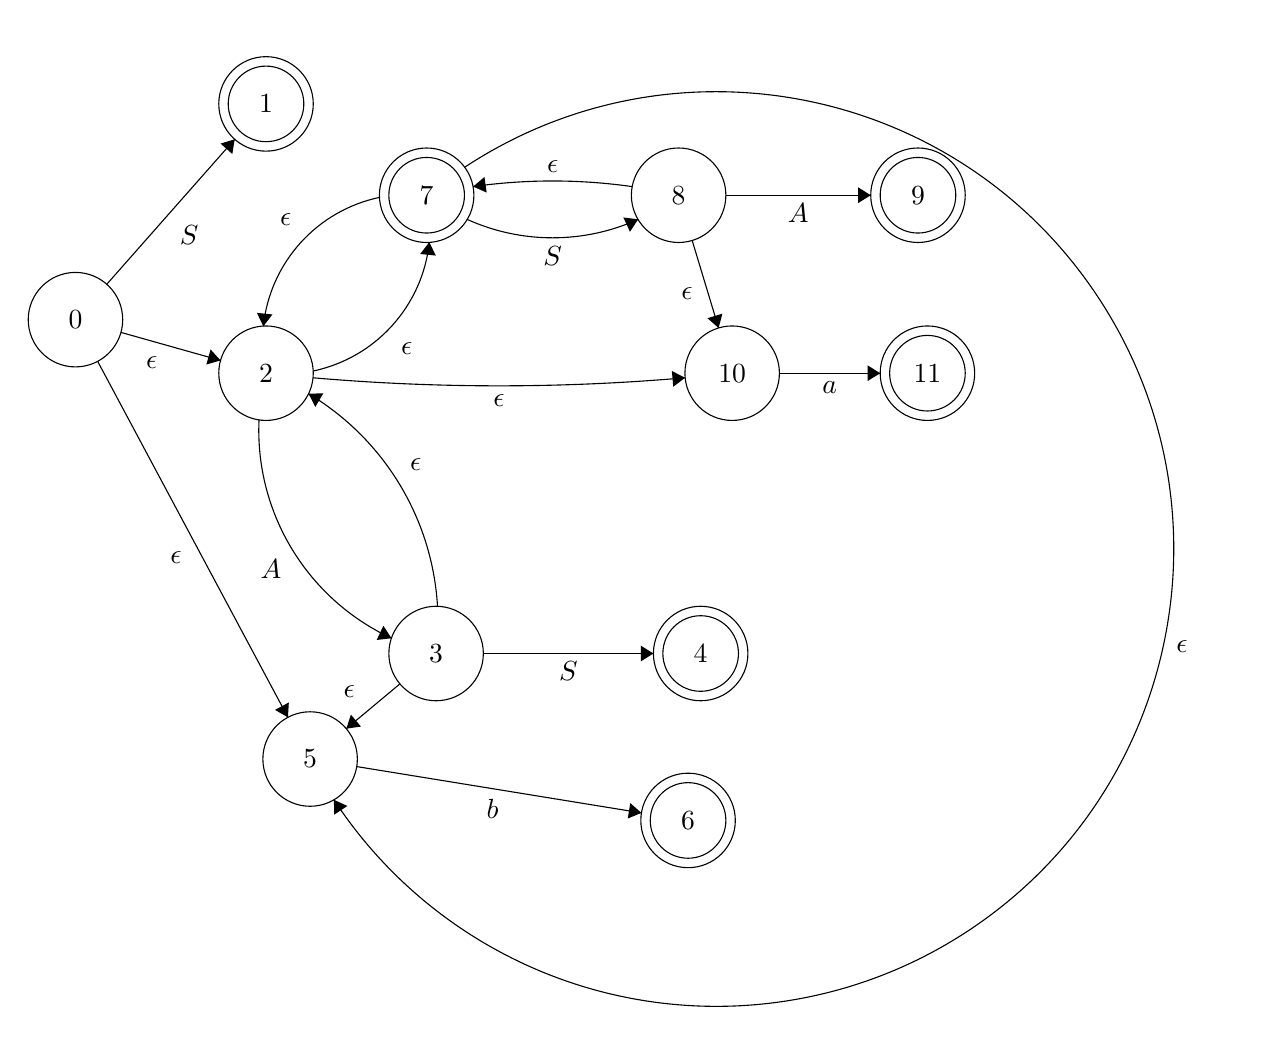
\begin{tikzpicture}[scale=0.2]
    \tikzstyle{every node}+=[inner sep=0pt]
    \draw [black] (8,-17.9) circle (3);
    \draw (8,-17.9) node {$0$};
    \draw [black] (47.7,-39.1) circle (3);
    \draw (47.7,-39.1) node {$4$};
    \draw [black] (47.7,-39.1) circle (2.4);
    \draw [black] (62.1,-21.3) circle (3);
    \draw (62.1,-21.3) node {$11$};
    \draw [black] (62.1,-21.3) circle (2.4);
    \draw [black] (61.5,-10) circle (3);
    \draw (61.5,-10) node {$9$};
    \draw [black] (61.5,-10) circle (2.4);
    \draw [black] (20.1,-4.2) circle (3);
    \draw (20.1,-4.2) node {$1$};
    \draw [black] (20.1,-4.2) circle (2.4);
    \draw [black] (46.9,-49.7) circle (3);
    \draw (46.9,-49.7) node {$6$};
    \draw [black] (46.9,-49.7) circle (2.4);
    \draw [black] (20.1,-21.3) circle (3);
    \draw (20.1,-21.3) node {$2$};
    \draw [black] (30.9,-39.1) circle (3);
    \draw (30.9,-39.1) node {$3$};
    \draw [black] (30.3,-10) circle (3);
    \draw (30.3,-10) node {$7$};
    \draw [black] (30.3,-10) circle (2.4);
    \draw [black] (46.3,-10) circle (3);
    \draw (46.3,-10) node {$8$};
    \draw [black] (49.7,-21.3) circle (3);
    \draw (49.7,-21.3) node {$10$};
    \draw [black] (22.9,-45.8) circle (3);
    \draw (22.9,-45.8) node {$5$};
    \draw [black] (9.99,-15.65) -- (18.11,-6.45);
    \fill [black] (18.11,-6.45) -- (17.21,-6.72) -- (17.96,-7.38);
    \draw (14.59,-12.5) node [right] {$S$};
    \draw [black] (9.41,-20.55) -- (21.49,-43.15);
    \fill [black] (21.49,-43.15) -- (21.55,-42.21) -- (20.67,-42.68);
    \draw (14.77,-33.02) node [left] {$\epsilon$};
    \draw [black] (19.93,-18.318) arc (-185.92867:-258.21361:9.345);
    \fill [black] (19.93,-18.32) -- (20.51,-17.57) -- (19.52,-17.47);
    \draw (21.75,-11.56) node [left] {$\epsilon$};
    \draw [black] (10.89,-18.71) -- (17.21,-20.49);
    \fill [black] (17.21,-20.49) -- (16.58,-19.79) -- (16.31,-20.75);
    \draw (12.85,-20.19) node [below] {$\epsilon$};
    \draw [black] (43.729,-11.534) arc (-65.69007:-114.30993:13.189);
    \fill [black] (43.73,-11.53) -- (42.79,-11.41) -- (43.21,-12.32);
    \draw (38.3,-13.2) node [below] {$S$};
    \draw [black] (49.3,-10) -- (58.5,-10);
    \fill [black] (58.5,-10) -- (57.7,-9.5) -- (57.7,-10.5);
    \draw (53.9,-10.5) node [below] {$A$};
    \draw [black] (30.469,-12.982) arc (-5.95024:-78.19204:9.348);
    \fill [black] (30.47,-12.98) -- (29.89,-13.73) -- (30.88,-13.83);
    \draw (28.65,-19.74) node [right] {$\epsilon$};
    \draw [black] (46.714,-21.592) arc (-85.04554:-94.95446:136.797);
    \fill [black] (46.71,-21.59) -- (45.87,-21.16) -- (45.96,-22.16);
    \draw (34.9,-22.6) node [below] {$\epsilon$};
    \draw [black] (33.249,-9.452) arc (98.12518:81.87482:35.74);
    \fill [black] (33.25,-9.45) -- (34.11,-9.83) -- (33.97,-8.84);
    \draw (38.3,-8.59) node [above] {$\epsilon$};
    \draw [black] (32.715,-8.222) arc (123.39605:-146.75362:29.041);
    \fill [black] (24.41,-48.39) -- (24.43,-49.33) -- (25.27,-48.78);
    \draw (77.88,-38.68) node [right] {$\epsilon$};
    \draw [black] (47.16,-12.87) -- (48.84,-18.43);
    \fill [black] (48.84,-18.43) -- (49.08,-17.52) -- (48.13,-17.81);
    \draw (47.23,-16.26) node [left] {$\epsilon$};
    \draw [black] (52.7,-21.3) -- (59.1,-21.3);
    \fill [black] (59.1,-21.3) -- (58.3,-20.8) -- (58.3,-21.8);
    \draw (55.9,-21.8) node [below] {$a$};
    \draw [black] (28.068,-38.126) arc (-114.88113:-182.62501:14.549);
    \fill [black] (28.07,-38.13) -- (27.55,-37.34) -- (27.13,-38.24);
    \draw (21.11,-33.75) node [left] {$A$};
    \draw [black] (22.798,-22.603) arc (59.13686:3.357:16.882);
    \fill [black] (22.8,-22.6) -- (23.23,-23.44) -- (23.74,-22.58);
    \draw (29.21,-27.07) node [right] {$\epsilon$};
    \draw [black] (28.6,-41.03) -- (25.2,-43.87);
    \fill [black] (25.2,-43.87) -- (26.13,-43.74) -- (25.49,-42.98);
    \draw (25.39,-41.96) node [above] {$\epsilon$};
    \draw [black] (25.86,-46.28) -- (43.94,-49.22);
    \fill [black] (43.94,-49.22) -- (43.23,-48.6) -- (43.07,-49.58);
    \draw (34.48,-48.34) node [below] {$b$};
    \draw [black] (33.9,-39.1) -- (44.7,-39.1);
    \fill [black] (44.7,-39.1) -- (43.9,-38.6) -- (43.9,-39.6);
    \draw (39.3,-39.6) node [below] {$S$};
    \end{tikzpicture}
    \end{center}
\begin{table}    
    \begin{tabular}{|c|c|c|c|c|}
    \hline
    & S & A & a & b \\
    \hline
    \{0, 2, 5, 7, 10\}& \{1, 2, 5, 7, 8, 10\} & \{2, 3, 5, 7, 10\} & \{11\} & \{6\} \\
    \hline
    \{1, 2, 5, 7, 8, 10\}& \{2, 3, 5, 7, 10\} & \{2, 3, 5, 7, 9, 10\} & \{11\} & \{6\} \\
    \hline
    \{2, 3, 5, 7, 10\}&\{2, 4, 5, 7, 8, 10\}  & \{2, 3, 5, 7, 10\} & \{11\} & \{6\} \\
    \hline
    \{2, 5, 7, 8, 10\}& \{2, 5, 7, 8, 10\} & \{2, 3, 5, 7, 9, 10\} & \{11\} & \{6\} \\
    \hline
    \{2, 3, 5, 7, 9, 10\}& \{2, 4, 5, 7, 8, 10\} & \{2, 3, 5, 7, 10\} & \{11\} & \{6\} \\
    \hline
    \{2, 4, 5, 7, 8, 10\}& \{2, 5, 7, 8, 10\} & \{2, 3, 5, 7, 9, 10\} & \{11\} & \{6\} \\
    \hline
    \{11\}& $\phi$ & $\phi$ & $\phi$ & $\phi$ \\
    \hline
    \{6\}& $\phi$ & $\phi$ & $\phi$ & $\phi$ \\
    \hline
    \end{tabular}
\end{table}
\begin{figure}[htbp]
    \centering
    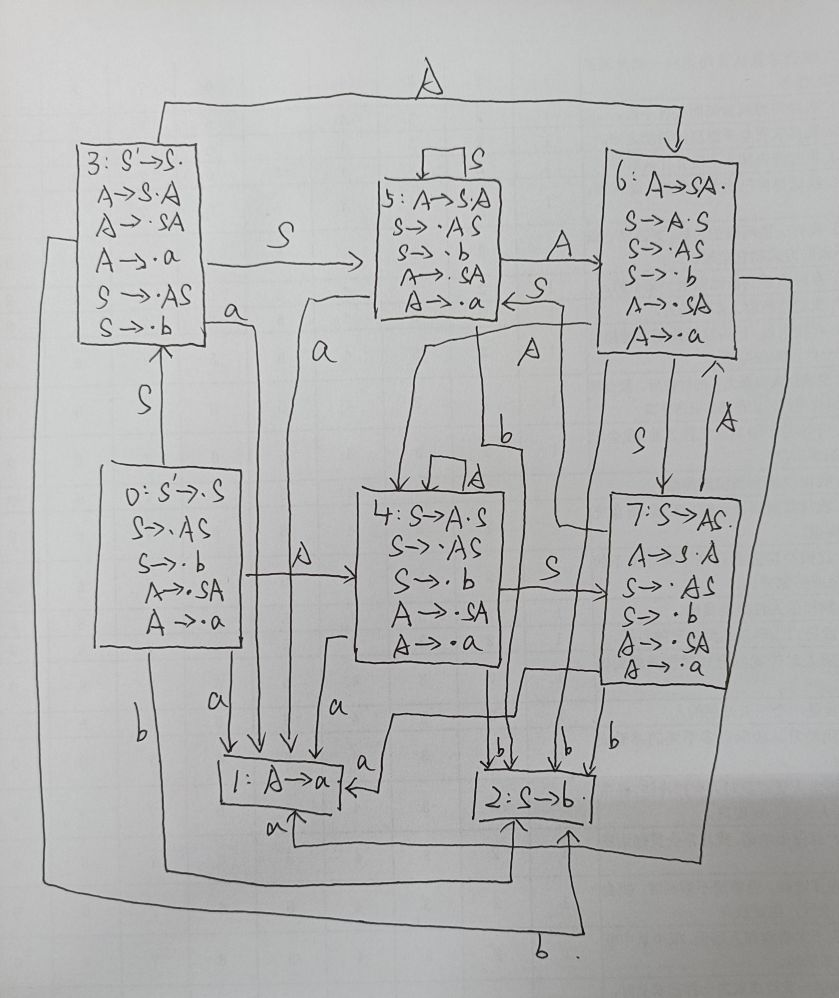
\includegraphics[scale=0.5]{4_1.jpg}
    \end{figure} 
项目集规范族见第5页.\\
\textbf{(3)}该文法不是SLR文法.\\
\textbf{证明:}显然,状态3、6、7有移进归约冲突,对于上述3个状态,分别有\\
FOLLOW(S’)=\{\#\},即a,b$\notin$FOLLOW(S’);\\
FOLLOW(S)=\{\#,a,b\},即a,b$\in$FOLLOW(S),则移进归约冲突无法消解;\\
FOLLOW(A)=\{a,b\},即a,b$\in$FOLLOW(A),则移进归约冲突消解.\\
综上所述,该文法不是SLR文法.\\
\textbf{(4)}首先构造LR(1)项目集规范族,考虑状态5,其包含项目[$A\rightarrow AS\cdot a/b$],
故遇到搜索符号a或b时,应通过$A\rightarrow AS$归约.\\
状态5包含项目[$A\rightarrow\cdot a a/b]$,故遇到搜索符号a时,应该移进.\\
因此存在“移进-归约”矛盾\\
所以,这个文法不是LR(1)文法.\\
\section*{5.7}
\noindent
由题意得,文法G[S]:  
0:S$\rightarrow$A\\  
1:A$\rightarrow$Ab\\  
2:A$\rightarrow$bBa\\  
3:B$\rightarrow$aAc\\  
4:B$\rightarrow$a\\  
5:B$\rightarrow$aAb\\    
显然,状态5有“归约-移进”冲突而状态9有“归约-归约”冲突,因此该文法不是LR(0)文法.  \\
对于状态5,有FOLLOW(B)=\{a\},故FOLLOW(B)$\cap$\{b\}=$\Phi$.\\ 
对于状态9,有FOLLOW(B)=\{a\},FOLLOW(A)=\{\#,b,c\},故FOLLOW(B)$\cap$FOLLOW(A)=$\Phi$.\\
因此状态5和状态9的冲突均可用SLR(1)方法解决,构造SLR(1)分析表可知该SLR(1)分析表无重定义.\\
因此该文法是SLR(1)文法,不是LR(0)文法.
\end{document}